\documentclass[licencjacka]{pracamgr}
\usepackage{polski}
\usepackage[utf8]{inputenc}
\usepackage[table]{xcolor}
\usepackage{array}
\usepackage{amssymb}
\usepackage{amsmath}
\usepackage{amsthm}
\usepackage[pdftex]{graphicx}
\usepackage{underscore}
\usepackage{hyperref}
\author{Tomasz Grabowski, Adam Markiewicz, Albert Rozmus, Krzysztof Rutkowski, Wiktor Zuba}
\nralbumu{305145, 334774, 248353, 319379, 320501}
\title{tytuł}
\tytulang{English title}
\kierunek{Informatyka}
\opiekun{dra Roberta Dąbrowskiego\\
Pion Zastępcy Kanclerza ds. Informatycznych}
\date{??? 2015}
\dziedzina{
11.0 Matematyka, Informatyka:\\
11.3 Informatyka\\
}
\klasyfikacja{
Information systems\\
Information systems applications\\
Decision support systems\\
Data analytics
}
%\TODO dodać litery/numery wierzchołków w klasyfikacji
\keywords{słowa kluczowe}
%\newtheorem{defi}{Definicja}[section]
\begin{document}
\maketitle
\begin{abstract}
Tu będzie abstract (skrót)
\end{abstract}
\tableofcontents
\chapter*{Wstęp}

Celem projektu było stworzenie serwisu internetowego zintegrowanego z systemem USOS 
wspierającego studentów w procesie świadomego doboru przedmiotów i konstruowania spójnego planu zajęć oraz
umożliwiającego studentom lepsze planowanie ścieżki studiów i kariery zawodowej
poprzez proponowanie przedmiotów, które mogą pasować do upodobań konkretnego studenta ocenionych na podstawie dotychczas wybieranych przedmiotów i otrzymywanych z nich ocen.
Dodatkowym wymaganiem projektu było oferowanie usług przewidywania dla konkretnych studentów ocen z przedmiotów, których jescze nie ukończyli lub nawet nie podjęli,
oraz przewidywania dla uniwersytetu ilości studentów którzy zapiszą się na konkretny przedmiot.
\addcontentsline{toc}{chapter}{Wprowadzenie}
 \chapter{Architektura}
TODO - lepszy obrazek \newline
 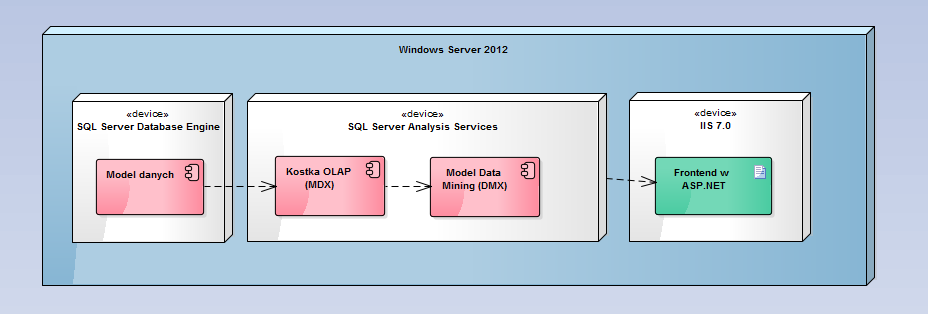
\includegraphics[scale=0.6]{Architektura.png}\newline
Chmura - Sercem systemu jest główny serwer znajdujący się w chmurze internetowej. Znajduje się na niej serwer bazy danych a także serwer WWW \newline
RDB - Relacyjna baza danych zawierająca statystyczne dane dotyczące zdawalności przedmiotow przez studentów, ich zapełnienia, popularność itd. Stanowi bazę do stworzenia kostki predykcyjnej. \newline
Analysis Services - usługi analityczne dokonujące analizy danych za pomocą algorytmów uczenia maszynowego oraz data mining. W naszym systemie służą do zamodelowania kostki analitycznej. \newline
Kostka OLAP -  kostka analityczna za pomocą której w naszym serwerze są obliczane i udostępniane predykcje. \newline
USOS Api - API udostępniane przez system USOS. Nasz system wykorzystuje go w celu zebrania danych zalogowanego użytkownika niezbędnych do wykonania poprawnych, możliwie celnych predykcji. \newline
Strona WWW - interfejs za pomocą którego użytkownik może przesyłać prośby o wykonanie udostępnianej przez system predykcji. \newline
Serwer WWW udostępniający użytkownikom stronę internetową, w naszym systemie pośredniczy między interfejsem użytkownika a kostką analityczną.  \newline
\newpage
Schemat działania i komunikacji między poszczególnymi komponentami :
1) Na samym początku działania system tworzy relacyjną bazę danych zawierającą dane statystyczne z USOSa. \newline
2) Po stworzeniu bazy danych system wykorzystuje usługi Analysis Services w celu stworzenia kostki analitycznej dokonującej predykcji i udostępnia ją serwerowi WWW. \newline
3)Po udanym stworzeniu kostki aktywuje się serwer WWW i system staje się dostępny dla użytkowników. \newline
4) użytkownik wchodzi na stronę i wysyła żądanie na serwer WWW \newline
5)Serwer WWW generuje stronę z formularzem zalogowania się \newline
6)Po odebraniu danych logowania, w przypadku udanego zalogowania Serwer pobiera dane użytkownika przez USOS Api i zwraca stronę WWW - interfejs użytkownika. \newline
7)Serwer WWW po odebraniu prośby o predykcje przesyła żądanie do kostki OLAP-owej (bazodanowego serwera?) o dokonanie predykcji wykorzystując odebrane wcześniej dane użytkownika. \newline
8)Serwer WWW odbiera rezultat zapytania i wyświetla go użytkownikowi. \newline

 \chapter{Technologia}
to tylko testowa wersja, pewnie ze wzgledu na duze przeciecie zdan z architektura bedzie potem do kosza ale kto wie \newline
Azure - Azure jest komercyjną platformą obsługiwaną przez Microsoft. Udostępnia ona usługi związane z chmurą internetową (tzw cloud-computing). W naszym systemie znajduje sie na niej serwer WWW a także serwer bazy danych. \newline
SQL Server 2014 - Komercyjny serwer bazodanowy udostępniany przez Microsoft. Znajduje się w nim relacyjna baza danych zawierająca dane niezbędne do stworzenia modelu analitycznego. \newline
SQL Server Analysis Services - usługi analityczne udostępniane przez SQL Server. W naszym systemie modelują kostkę OLAP-ową służącą do predykcji a także udostępniają ją serwerowi WWW. \newline
USOS Api - API udostępniane przez system USOS. Nasz system wykorzystuje go w celu zebrania danych zalogowanego użytkownika niezbędnych do wykonania poprawnych predykcji. \newline
Serwer WWW udostępniający interfejs użytkownika - stronę WWW wykonaną w technologii ASP.NET. W celu uzyskania możliwie dużej przenośności została zaprojektowana w metodologii RWD (Responsive Web Design).  \newline
\begin{thebibliography}{99}
\addcontentsline{toc}{chapter}{Bibliografia}
\bibitem[abc]{ABC} Książka 1
\bibitem[def]{DEF} Link 2
\end{thebibliography}
\end{document}